This chapter provides a brief overview of combustion theory. The discussion is limited to some of the concepts used in the following chapters. The aim is to provide the necessary ingredients to model combustion phenomena mathematically. We begin by introducing some basic terms such as premixed flames, diffusion flames and partially premixed flames in section \ref{sec:background:classifications}. Subsequently, we present in section \ref{sec:background:math} the mathematical equations that describe flame propagation in a flow field.

\section{Review}\label{sec:background:classifications}


In addition to the significance of flame balls as a possible mode of combustion in weakly flammable mixtures,
an important related aspect, of particular relevance to the present work, is their significance  in ignition problems involving heat addition  by  an external source  such  as an electric spark. In this context, they may indeed serve to estimate the minimum energy to be deposited by the source for successful ignition whereby an initially formed  hot kernel   generates an outwardly propagating  flame front \cite[p.~331]{zeldovitch_math_theory}. For successful ignition to occur, however, both the power and the duration of the source need   be taken into account \cite{Joulin1,Joulin2,Joulin4}. In the particular case of a point source of constant power, two branches of stationary solutions are obtained depending on the power of the source \cite{Joulin1}; the lower branch representing small flame balls  being stable, the upper branch  representing large flame balls, including  Zeldovich flame balls, being unstable.

In this work, we extend these studies, by considering a model for flame balls in the presence of a flow of hot inert gas, either a source or a sink, at their origin. Depending on the direction and magnitude of the flow, these flames
can have positive, zero or negative burning speeds, with zero  speeds characterising  Zeldovich  flame balls. We shall refer to these stationary solutions of the advection-diffusion-reaction heat and mass transport equations as   \emph{generalised flame balls}.

One motivation for studying these solutions is that they provide a simple framework  for analysing the important problem of flame initiation, intentional or accidental, by a hot gas stream \cite[p.~265]{williams_combustion_Theory}-\cite{Sadanandan}.  They also provide valuable analytical information on the effect of convection, albeit for a specific radial flow,  on the existence and stability of flame balls. Finally, the dependence of their burning velocity, positive or negative, on their curvature, small or large,  may provide some insight into such dependence  when studying the local behaviour of more complex premixed flames such as edge-flames in strained mixing layers or flamelets in    turbulent flow fields.

This chapter is structured as follows. We begin by formulating the model  and identifying its main non-dimensional parameters.  An asymptotic analysis is then presented, where the  stationary solutions, their multiplicity and their stability  are fully described. This is  followed  by a numerical study  which validates and illustrates the analytical
results.  Finally, a conclusion section where the main findings are summarised and  additional extensions of the work  suggested, closes the chapter.

\section{Mathematical formulation}\label{sec:background:math}

\begin{figure}[]
 \centering
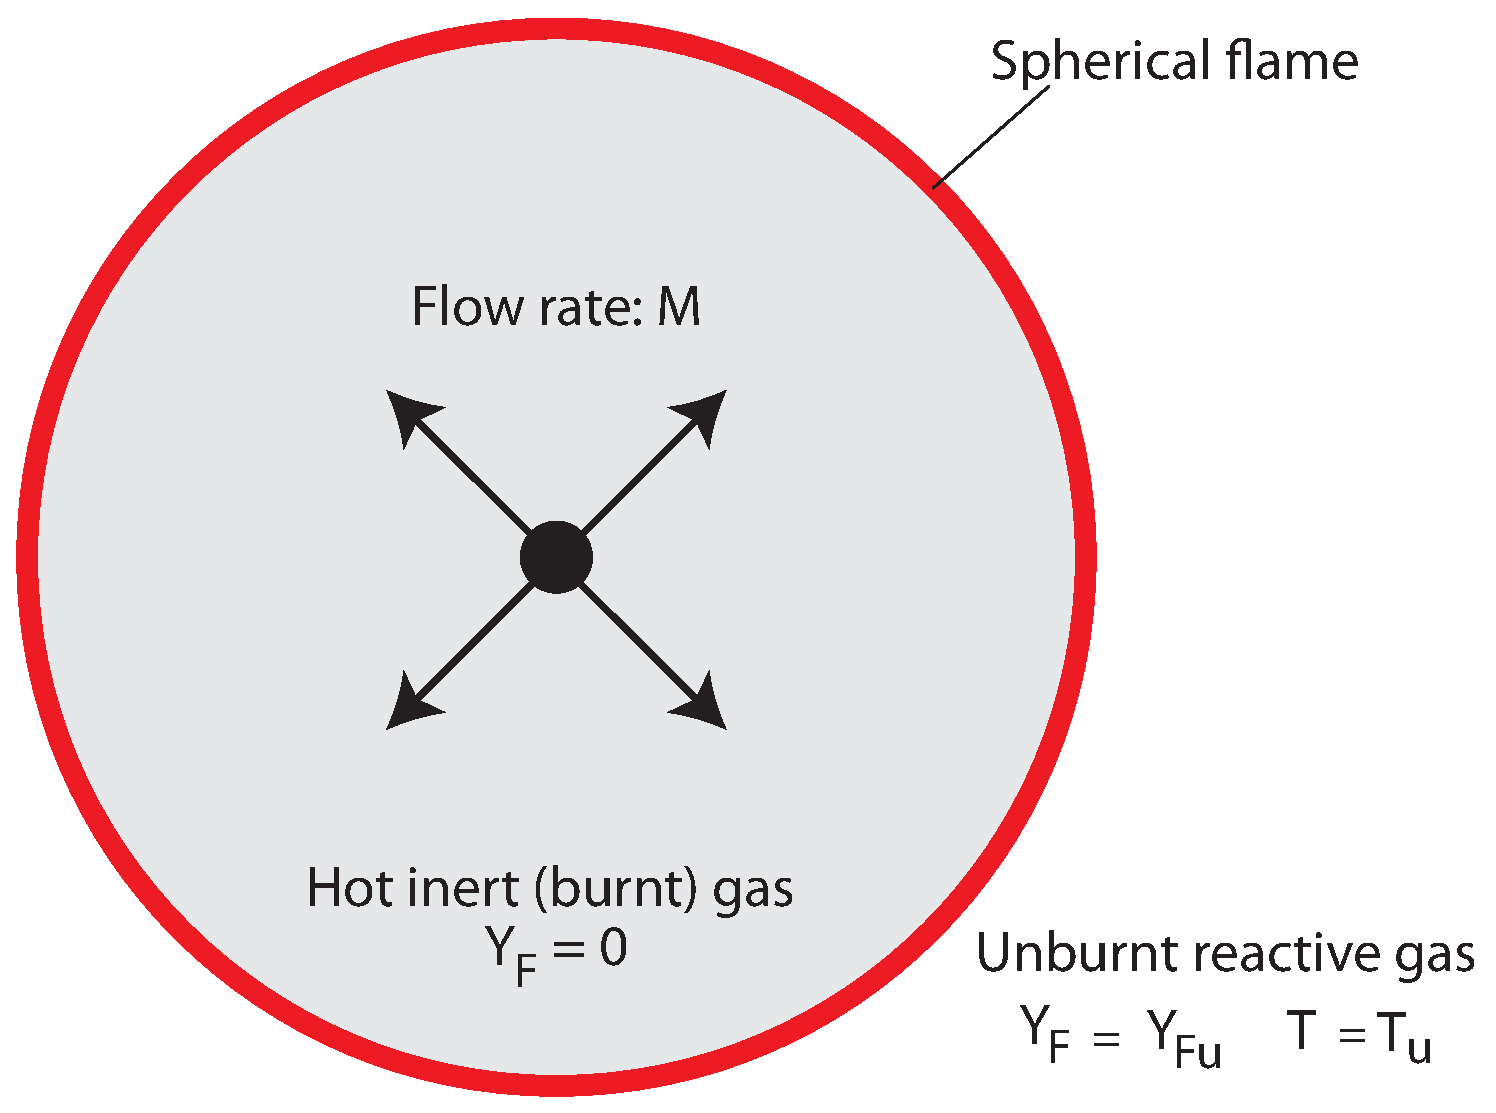
\includegraphics[width=0.6\textwidth]{Configuration.eps}
\caption{ Spherical flame sustained by a point source
of hot inert gas, with flow rate $M>0$. Negative values of $M$
correspond to a sink (not shown in this figure).}
\label{Configuration}
\end{figure}

We consider a spherically symmetric flame around a point source of
hot inert gas located at the origin, as shown in figure~\ref{Configuration}. The governing equations can be written in spherical coordinates using the conservation equations presented in Chapter 2. Within the thermo-diffusive
approximation of constant density and constant transport properties,
a relevant non-dimensional model consists of the equations
\begin{eqnarray}
&&\label{eqn:num:theta}\frac{\partial{\theta}}{{\partial t}}+
\frac{M}{r^2}\frac{\partial{\theta}}{{\partial r}}=\frac{1}
{r^{2}}\frac{\partial}{\partial r} (r^{2}\frac{
\partial{\theta}}{{\partial r}})+ \omega,
\\
&&\label{eqn:num:yF}\frac{\partial{y_{F}}}{{\partial t}}+
\frac{M}{r^2}\frac{\partial{y_{F}}}{{\partial
r}}=\frac{1}{\Le}\frac{1} {r^{2}}\frac{\partial}{\partial r}
(r^{2}\frac{
\partial{y_{F}}}{{\partial r}})- \omega,
\end{eqnarray}
subject to the  far-field boundary condition
\begin{eqnarray}
&&\label{eqn:num:cond:R}\theta=0, \quad \quad y_{F}=1 \quad \quad
\text{as }\quad r\rightarrow \infty,
\end{eqnarray}
and the requirement inside the ball that
\begin{eqnarray}
&&\label{eqn:num:cond:Lg}
\begin{cases} (\theta,y_F)=(\theta_0,0) &\quad  \text{for } \quad M>0  \\
 (\theta,y_F)\, \text {are bounded}  &\quad  \text{for} \quad  M\leq 0
\end{cases}  \quad \quad \text{as } \quad r\rightarrow 0\,.
\end{eqnarray}

Here $\theta$ and $y_{F}$ are the non-dimensional  temperature and
mass fraction of the fuel, respectively, and $\Le$ is the Lewis
number of the fuel.  They are given by $\theta = (T-T_u)/(T_{ad}-T_u)$ and $y_F
= Y_F/ Y_{Fu}$, where $T_u$ and $Y_{Fu}$ are the temperature and the
fuel mass fraction of the  reactive mixture in the far-field, and
$T_{ad}$ is the adiabatic \emph {planar flame} temperature. The fuel
is assumed to   limit the reaction rate $\omega$, which is taken to
follow the standard (non-dimensional) Arrhenius form
\[ \omega =
\frac{\beta^{2}}{2 \Le} y_{F} \exp\left(\frac{\beta
(\theta-1)}{1+\alpha(\theta-1)}\right),
\]
where $\beta$ is the non-dimensional activation energy or Zeldovich
number, and $\alpha=(T_{ad}-T_{u})/T_{ad}$ the heat release parameter.
A convection term of strength $M$  is included in the equations to
account for the presence of  point-source radial flow  at the origin if $M>0$, where $M$ represents the
non-dimensional volumetric flow rate; when $M<0$, we are in the presence of a sink which sucks the burnt gas. The units for speed and length chosen for the non-dimensionalisation correspond to
the propagation speed $S_{L}$  and the thickness $\ell_{Fl}$ of the
\emph{planar flame} (more precisely to the asymptotic values of
these as $\beta \rightarrow \infty$, which are discussed in Chapter 2).

The far-field boundary condition (\ref{eqn:num:cond:R}) corresponds
to a frozen mixture with prescribed temperature and composition. The
boundary condition (\ref{eqn:num:cond:Lg}) specifies the temperature
of the fuel-free (inert) stream at the origin when $M>0$; this
condition is redundant when $M \leq 0$ if $\theta$ and $y_F$ are
simply required  to be bounded.

We have now completed the formulation of the problem. The main task
is to find time-independent solutions to equations
(\ref{eqn:num:theta}) to (\ref{eqn:num:cond:Lg})  which represent spherical
flame balls  whose radius $R$ depend on the parameters $\Le$, $M$
and $\theta_0$,  in addition to $\beta$ and~$\alpha$.


We begin by reformulating the problem in the asymptotic limit $\beta
\rightarrow \infty$ in the next section. This is followed by an
analytical treatment  which allows $R$ to be determined in terms  of three parameters representing $\Le$, $M$ and $\theta_0$, along with
the multiplicity of the solutions. The linear stability of these to one-dimensional perturbations
is then addressed analytically. Finally, a numerical treatment
of the problem with a finite value of $\beta$ is provided, which supports and illustrates the analytical findings.  We also
discuss the application of the  results to the problem of ignition by a hot inert gas flow  and to clarifying
the dependence of the speed and the burning rate of the  flames encountered on their curvatures. 